% Publication: EIDORS: uses and abuses
% Authors: Andy Adler, Bill Lionheart
% $Id: adler-lionheart-2005-EIDORS.tex,v 1.7 2005-11-01 04:01:26 aadler Exp $
\documentclass[12pt]{iopart}
\usepackage[dvips]{graphicx} % Package for inserting figures
\begin{document}
\title{Electrial Impedance and Diffuse Optical
       Tomography Reconstruction Software (EIDORS) version 3: uses and abuses}
\author{Andy Adler$^1$, William R. B. Lionheart$^2$}
\address{$^1$ School of Information Technology and Engineering (SITE), University of Ottawa, Canada}
\address{$^2$ School of Mathematics, University of Manchester, U.K.}
\eads{
   \mailto{adler@site.uOttawa.ca}
   \mailto{bill.lionheart@manchester.ac.uk}
     }

\begin{abstract} %Single paragraph text only (no ref. eqn. max.200 words)

EIDORS is an open source software suite for image reconstruction in
electrical impedance tomography and diffuse optical tomography;
designed to facilitate collaboration, testing and new research
in these fields.  This paper describes recent work to
redesign the software structure in order to simplify its use
and provide a uniform interface,
permitting easier modification and customization.
We describe the key features of this software, followed by
examples of its use.
One general issue with inverse problem software, is the difficulty
of correctly implemeting algorithms, and the consequent ease with
which subtle numerical bugs can be inadvertently introducted.
EIDORS helps with this issue, by allowing sharing and reuse
of well documented and debugged software. On the other hand, 
EIDORS potentially encourages such issues by facilitating use
by non-specialists. In order to address this issue, we develop
a list "cheats with inverse problems". Our hope is that such
a list will assist authors of software to avoid such implemention
issues.


\end{abstract}
\noindent{\it Keywords\/}:
Electrical Impedance Tomography,
Open Source,
Inverse Problems

\section{Introduction}

EIDORS3D is a software suite for image reconstruction in
electrical impedance tomography and diffuse optical tomography.
The goal is to provide a freely distributable and modifyable
software for image reconstruction of electrical 
or diffuse optical data. Such software facilitates research
in these fields by providing a reference implementation
against which new developments can be compared, and by
providing a functioning software base onto which new
ideas may be built and tested.
The original EIDORS software (Vaukhonen et al., 2000) 
is based on software from the thesis of Vaukhonen (1997)
It implemented a MATLAB package for two-dimensional mesh generation,
solving of the forward
problem and reconstruction and display of the images.
In order to provide capability to solve 3D reconstruction models,
a new project, EIDORS3D, was begun (Polydorides and Lionheart, 2002),
based on the software developed for thesis of Polydorides (2002).
The EIDORS software packages shared the same numerical
foundations; media are modelled using a finite element representation,
and the images are reconstructed using regularized inverse techniques.

In the three years since the publication of EIDORS3D, several patterns
of use have been noted. Researchers typically download the software,
run the provided demonstration examples,  and 
make modifications in the demonstration examples and the software
internals to meet their needs.
Because of the lack of a modular software structure of EIDORS3D,
changes tended to made into the code itself. This resulted in
duplicated
code which could not easily be <i>refactored</i> in order to
be contributed back to EIDORS3D. Additionally, recent work has begun to move
away from basic reconstruction algorithms, focussing
on such issues as mesh generation, electrode modelling, visualization
and electrode error detection. This research would be facilitated
by using modular components which could be <i>plugged</i> into
a selection of reconstruction algorithms.

To address these issues, the EIDORS3D software has been completely
restructured with the goal of providing an {\em extensible software base}
designed to support {\em community} use, modification and contribution.
This has been accomplished by the following:

\begin{itemize}

  \item {\em Open-source license:}
EIDORS3D is licensed under the
GNU General Public License. Uses are free to use, modify, and
distribute their modifications. All modifications must include the
source code, or instructions on how to obtain it. EIDORS3D may be used
in a commercial product, as long as the source code for EIDORS and all
modifications to it are made available.

  \item {\em Sourceforge hosting:}
EIDORS is hosted by {\tt sourceforge.net}
at {\tt http://eidors3d.sf.net}.
Software is available for download as packaged released versions
(version 3.0 was released on 28 Oct 2005, and
contains the features described in this paper),
or the latest developments may be downloaded from the CVS
version control repository.
Sourceforge hosting allows for collaborative development for
group members, while permitting read-only access to everyone.
In order to become a member of the developer group, new
contributors should contact the authors.

  \item {\em Language independence: (Octave and Matlab)}
EIDORS3D was originally written for Matlab.
However, the eventual goal is for language independence.
The current version of EIDORS3D works with Octave
({\em www.octave.org}, version $\ge$ 2.9.3)
and Matlab (version $\ge$ 6.0).
Since Octave is free software, EIDORS could be provided
as part of an EIT system without incurring the additional
licensing costs of Matlab.

  \item {\em Pluggable code base:}
In order to facilitate user modifications, EIDORS3D
has been designed to provide some of the benefits of
Object-oriented (OO) software: {\em Packaging}
 and {\em Abstraction}. We have decided not to
use the OO framework provided by Matlab, because
it appears somewhat cumbersome, and may be intimidating
to many mathematicians and engineers who do not 
regularly write OO software. This decision may
be revisited in the future.
Instead, EIDORS has been designed as 
"Pluggable" software. This design uses function
pointers to allow adding new modules and controlling
which parts of functions are executed.
A detailed description of this capability is
provided in the next section.

  \item {\em Automatic matrix caching:}
In order to increase
performance of image reconstruction software, it is important to cache
computationally expensive variables, such as the Jacobian and image priors.
Such caching
complicates the software implementation. To solve this problem,
EIDORS3D extracts caching to a separate module {\em eidors\_obj}
which is inherited by
each functional module. This capability is described in the next section.

  \item {\em Generalized data formats:}
In order to support the wide
variety of EIT measurements and algorithms, a general EIT data format
structure is developed (the {\em fwd\_model} structure).
This format specifies the electrode positions, contact impedances,
and stimulation and measurement patterns.

  \item {\em Interface software for common EIT systems:}
Functions
to load data from some common EIT systems to the EIDORS3D data
format have been developed.
As coverage of more data formats is implemented, 
we hope that this will advance the ability of researchers
to share data and results.

  \item {\em Usage examples:}
It is observed that researchers typically base new software on
demonstration examples. To facilitate this, some simple and more
complex usage examples are provided.

  \item {\em Test suite:}
Software is intrinsically difficult to test. While little work
has been done specifically on testing numerical software, we
believe that such tests are even more difficult.
EIDORS3D has begun to implement a series of regression test
scripts to allow automatic testing of code modifications.

  \item {\em Enhanced Finite Element Modelling and Graphical output:}

  \item {\em Logo:}
Since EIDORS images blobby objects in aqueous media,
the logo \label{fig:logo}, was chosen to be a walrus; it is (also)
a fat, blobby animal that lives in water.

%
% FIGURE: EIDORS LOGO
%
\begin{figure}[th]
\begin{flushright}
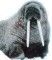
\includegraphics[width= 0.30 \textwidth]{./eidors-logo.eps}
\caption{\small EIDORS logo.
{\em EIT}: images blobby objects in aqueous media;
{\em Walrus}: a fat, blobby animal that lives in water.
 Images credit: www.biosbcc.net (C) Genny Anderson

{\tt TODO: Get a better picture}
 }


\end{flushright}
\end{figure}

\end{itemize}
We hope that by providing a structure for community collaboration
in EIT algorithms, we can produce robust,
reliable and fairly portable software which draws on our collective
expertise and facilitates innovations in the field.

\section{Software Architecture}

\subsection{Software Example: Calculation of the Jacobian}
In order to illustrate the usage of EIDORS3D, we consider
the calculation of the Jacobian, or sensitivity matrix,
$\bf J$
Given a finite element model (FEM) model of an EIT medium,
$F$, we calculate the vector of voltages, $\bf v$, 
at each FEM vertex as:
\begin{equation}
{\bf v} = F( \sigma ){\bf q} 
\end{equation}
where $\sigma$ is the vector of element conductivities
and $\bf q$ is the current stimulation pattern, a vector
of current inputs to each vertex (Neumann boundary conditions).
Depending on the electrode model used, the measured electrode
voltage can be represented as a linear combination of vertex
voltages, ${\bf V}_{2E}$.
For each simulation pattern, ${\bf }q_{i}$,
measurements $m_{i,j}$
are performed, each of which consist of a linear combination of
electrode measurements, ${\bf m}_j$.
Thus:
\begin{equation}
m_{i,j} = {\bf m}_{i} {\bf V}_{2E} F( \sigma )
\end{equation}
Based on this model, $\bf J$ is calculated as:
\begin{equation}
{\bf F}_{i,j,k} = \left.\frac{
 {\bf m}_{i} {\bf V}_{2E}{\partial}F( \sigma )
}{
{\partial}{\bf \sigma}_k
}
\right|_{
   {\bf \sigma} = {\bf \sigma}_0 
}
\end{equation}
where ${\bf \sigma}_0$ is the "background"
conductivity around which small changes are assumed to occur.
In EIDORS, the Jacobian is calculated using {\tt calc\_jacobian};
this function needs as parameters the FEM model {\tt fem},
of type $\tt fwd_model$,
and the image of the background {\tt img\_bkgnd}
of type {\tt image}.

\subsection{Forward Model structure {\tt fwd\_model} }

The following table shows a partial representation of 
the structure of an EIDORS3D {\tt fwd\_model} object.

\begin{tabular}{ll}
{\bf Properties} & {\bf Description } \\
\hline
{\tt
        fwd\_model.name
} &
        Model name (arbitrary)
\\
{\tt
        fwd\_model.nodes
} &
        Position of FEM vertices
        $n_V{\times}n_D$
\\
{\tt
        fwd\_model.elems
} &
        Node indices of FEM elements
        $n_N{\times}n_D+1$
\\
{\tt
        fwd\_model.boundary
} &
        Node indices of element faces on the medium surface
\\
{\tt
        fwd\_model.electrode
} &
        Vector $n_E{\times}1$
           of electrode models ({\tt elec\_model})
\\
{\tt
        fwd\_model.stimulation
} &
         Vector $n_S{\times}1$of stimulation
            patterns ({\tt stim\_model})
\\
\hline
{\bf Methods} & {\bf Description } \\
\hline
{\tt
        fwd\_model.solve
} &
        Function to calculate inverse solution
\\ &
        {\tt {\em data} = fwd\_solve( fwd\_model, {\em image} )}
\\
{\tt
        fwd\_model.jacobian
} &
        Function to calculate Jacobian at {\em image} background
\\ &
        {\tt {\em J} = calc\_jacobian( fwd\_model, {\em image} )}
\\
\end{tabular}


Each object is created using the {\tt eidors\_obj}
function, which can fill in default attributes, and 
keeps track of cached properties.
Given a {\tt fwd\_model} {\tt\em fem}
a background image may be defined as follows:
\begin{verbatim}
homg_conductivity= ones( length(fem.elems) ,1);
img_bkgnd= eidors_obj('image', 'homog background', ...
  'elem_data', homg_conductivity, 'fwd_model', fem );
\end{verbatim}
where the object {\tt name} is assigned
(arbitrarily) to 'homog background'.
In order to calculate the Jacobian, we call
{\tt J= calc\_jacobian( fem, img\_bkgnd )}, which
1). tests to see whether {\bf J} has been previously
calculated for {\tt fem} and {\tt img\_bkgnd}; if
so, the cached value is returned; otherwise,
2) loads and calls the function in {\tt fem.jacobian},
which may be {\tt np\_calc\_jacobian}, which 
calls the code from Polydorides (2002); the returned
value is then stored in the cache and returned to the
calling function.

\section{ Usage Examples}

In this section two examples of the usage of EIDORS3D
software functions are provided. The first illustrates
the use of forward models to simulate data. The second
illustrates how to modify the image reconstruction
behaviour of an existing algorithm to
add new features without needing to edit the original
software.

\subsection{ Simulate Data }
In order to simulate data, a FEM model object {\tt mdl\_3d}
and a conductivity image need to be created.
\begin{verbatim}
% mk_circ_tank(FEM_rings, FEM_levels, n_elec, elec_planes )
param= mk_circ_tank(8, [-1:.25:1], 16, 3);

% mk_stim_patterns(n_elec, elec_planes, stim, meas, opt, stim_amplitude)
options = {'no_meas_current','no_rotate_meas'};
params.stimulation= mk_stim_patterns(16, 3, '{ad}','{ad}', opt, 10);

params.solve=      'np_fwd_solve';
mdl_3d = eidors_obj('fwd_model', params);
show_fem( mdl_3d );  % View model

% simulate using <i>img_bkgnd</i> above
homg_data=fwd_solve( mdl_3d, img_bkgnd);
\end{verbatim}

The functions {\tt mk\_circ\_tank} and {\tt mk\_stim\_patterns}
build regular cylidrical EIT FEM models. In order to use more
sophisticated simulations, these functions can be replaced
by the user. For example, code to build models using {\em netgen}
{\tt http://www.hpfem.jku.at/netgen/} is available in the
{\tt meshing/netgen/} directory.

\subsection{  Reconstruct Images }

This example shows how modify an existing algorithm.
For example, we wish to modify the
hyperparameter selection strategy of Polydorides (2002) to use
instead the {\em Noise Figure} parameter introduced by
Adler and Guardo (1996). The first step is to create a
{\tt fwd\_model} structure {\em demo\_mdl} in a similar
way to the above (details are shown in {\tt examples/demo\_real.m}).
Subsequently, an {\tt inv\_model}, {\tt demo\_inv} is created,
and the image reconstructed from difference data: 
{\tt data1} and {\tt data2}.

\begin{verbatim}
demo_inv.name= 'Nick Polydorides - Modified';
demo_inv.solve= 'np_inv_solve';
demo_inv.reconst_type= 'differential';
demo_inv.fwd_model= demo_mdl;

% modify to use Tikhonov prior
demo_inv.image_prior.func= 'tikhonov_image_prior';

% modify to use Noise Figure of 2.0
demo_inv.hyperparameter.func = 'aa_calc_noise_figure';
demo_inv.hyperparameter.noise_figure = 2.0;
demo_inv= eidors_obj('inv_model', demo_inv);

% solve inverse
solve_img= inv_solve( demo_inv, data1, data2);
\end{verbatim}

\section{
 Example: modifying electrode configuration for 3D model
}

%
% FIGURE: Zigzag electrode config
%
\begin{figure}[th]
\begin{flushright}
\includegraphics[width= 0.80 \textwidth]{./fig_3d.eps}
\caption{\small The 
{\em Modification of NP's model to use 16 electrodes in a
zig zag configuration and reconstruction with them}
 \label{fig:fig_3d}
}
\end{flushright}
\end{figure}

\section{
 Cheating with EIT
}

In this section, we try to point out some
simple approaches that work with common, linear
regularization techniques. As the solution
strategy becomes more complex, then clearly there
become more advanced ways to cheat.

\subsection{
Sample Problem: The happy transform
}
To motivate the problem, assume that EIT measurement
data have been acquired from an image which resembles
a 'sad' face. Being of an optimistic outlook, we wish
that the image reconstructed represent a 'happy' face
instead. Fig. \ref{fig:happytransform}
illustrates this ``happy transform''.

%
% FIGURE: Happy Transform
%
\begin{figure}[th]
\begin{flushright}

\includegraphics[width= 0.30 \textwidth]{./sad.eps}

\includegraphics[width= 0.30 \textwidth]{./happy.eps}
\caption{\small The 
{\em happy transform}
 }
 \label{fig:happytransform}
\end{flushright}
\end{figure}

\subsection{ Cheating approach \#1:
 Careful selection of noise }

Typically, a reconstruction algorithm is presented
with white Gaussian noise (WGN) added to the data. One
technique to perform the happy transform is to
carefully select the noise.
In this case, we simulated a homogenous (${\bf v}_h$)
and inhomogeneous (${\bf v}_i$) data on a 256
element FEM. Subsequently 17.75dB of WGN was added to
${\bf v}_i$, and the images reconstructed using
the algorithm of Adler and Guardo (1996).
Each image was reconstructed (with different selections of
hyperparameter values), and reviewed by the author to determine which cases
corresponded to the happy transform.
Fig. \ref{fig:happynoise} shows two successful
``happy'' images.

%
% FIGURE: Happy Noise
%
\begin{figure}[th]
\begin{flushright}
\includegraphics[width= 0.50 \textwidth]{./fig_noise.eps}
\caption{\small 
Images with 17.75dB WGN which were selected as ``happy''
 }
 \label{fig:happynoise}
\end{flushright}
\end{figure}

In order to determine the frequency of 'happy' noise, 2000
images were reviewed and 41 were selected, corresponding
to an occurance rate of approximately 2\%.
While careful noise selection is not a mathematical/computational
technique, it is commonly used in association in research,
and thus merits mention here.

\subsection{ Cheating approach \#2:
             Careful selection of priors}

The Bayesian framework for regularization interprets
the image penalty term as {\em a priori} information 
about the underlying image probability distribution.
In practice, however, this term is selected using
ad hoc or heuristic techniques. If the prior does
not correspond to the real case, then the reconstructed
image will be biased. This idea is key for approach \#2.

In a Tikhonov regularization scheme, image amplitude
is penalized. We use the following formulation:
\begin{equation}
   \hat{\bf x} = 
   \left({\bf H}^t{\bf H} + \lambda{\bf R}\right)^{-1}
         {\bf H}^t{\bf y}
\end{equation}
where the regularization term 
\begin{equation}
   {\bf R} = \sqrt{ trace {\bf H}^t{\bf H} }
\end{equation}

If, however, we {\em know} {\em a priori} that 
our data were measured from a happy face, then we 
would not wish to penalize image pixels which we
{\em know} to be large. Thus for each pixel {\em i}
in the happy face, we set 

\begin{equation}
   {\bf R}_{i,j} = \frac{1}{2} \left[
              \sqrt{ trace {\bf H}^t{\bf H} }
                               \right]_{i,j}
\end{equation}

The effect of careful prior selection is hown in
Fig. \ref{fig:tikprior}.
In this case, images were reconstructed on a 576 element
FEM (chosen to differ from the 256 element simulation mesh).


%
% FIGURE: Tikhonov Prior
%
\begin{figure}[th]
\begin{flushright}
\includegraphics[width= 0.80 \textwidth]{./fig_tik_wo-icrime.eps}
\caption{\small 
Reconstructed images illustrating the effect of image priors,
using different mesh for model and reconstruction.
Images are numbered from left to right.
{\em Image 1:} Tikhonov prior with no weighting,
{\em Image 2:} Tikhonov prior with weighting for positions in sad face,
{\em Image 3:} Tikhonov prior with weighting for sad face (left) and
happy face (right),
{\em Image 4:} Tikhonov prior with weighting for positions in happy face,
 }
 \label{fig:tikprior}
\end{flushright}
\end{figure}

In order to enhance this effect, we use an {\em inverse crime},
by putting the Tikhonov prior information {\em exactly} where
it needs to be to get the happy face (Fig. \ref{fig:tikprior_icrime}).

%
% FIGURE: Tikhonov Prior with inv crime
%
\begin{figure}[th]
\begin{flushright}
\includegraphics[width= 0.80 \textwidth]{./fig_tik_w-icrime.eps}
\caption{\small 
Reconstructed images illustrating the effect of image priors,
using {\em same} mesh for model and reconstruction.
Images are numbered from left to right.
{\em Image 1:} Tikhonov prior with no weighting,
{\em Image 2:} Tikhonov prior with weighting for positions in sad face,
{\em Image 3:} Tikhonov prior with weighting for sad face (left) and
happy face (right),
{\em Image 4:} Tikhonov prior with weighting for positions in happy face,
 }
 \label{fig:tikprior_icrime}
\end{flushright}
\end{figure}


\subsection{ Cheating approach \#3:
             Edge based priors}

It is somewhat difficult to properly model a Laplacian filter
on a Finite Element mesh, but one way to approximate it is to
do the following: for each edge between elements $i$
and $j$, put 1 at $i,i$ and $j,j$
and $-1$ at $i,j$ and $j,i$.

Such a Laplacian filter can be used as a regularization prior
to penalize high frequency components (edges) in the image.
On the other hand, if we {\em know} where the edges are,
then edges should not be penalized (or be less penalized) in
those places. Fig \ref{fig:laplprior}
shows the effect of such careful
edge preserving prior selection (with no {\em inverse crime}).
{\em Known edges} are weighted at $0.3\times$ that of other
edges in the image.

%
% FIGURE: Laplace prior
%
\begin{figure}[th]
\begin{flushright}
\includegraphics[width= 0.80 \textwidth]{./fig_lapl_wo-icrime.eps}
\caption{\small 
Reconstructed images illustrating the effect of edge
preserving image priors,
using different mesh for model and reconstruction.
Images are numbered from left to right.
{\em Image 1:} Edge prior with no weighting,
{\em Image 2:} Edge prior with weighting for positions in sad face,
{\em Image 3:} Edge prior with weighting for sad face (left) and
happy face (right),
{\em Image 4:} Edge prior with weighting for positions in happy face,
 }
 \label{fig:laplprior}
\end{flushright}
\end{figure}

In order to enhance this effect, we use an {\em inverse crime},
by putting the Tikhonov prior information {\em exactly} where
it needs to be to get the happy face
(Fig. \ref{fig:laplprior-icrime}).
{\em Known edges} are weighted at $0.3\times$ that of other
edges in the image.

%
% FIGURE: Laplace prior with inv crime
%
\begin{figure}[th]
\begin{flushright}
\includegraphics[width= 0.80 \textwidth]{./fig_lapl_w-icrime.eps}
\caption{\small 
Reconstructed images illustrating the effect of edge
preserving image priors,
using same mesh for model and reconstruction.
Images are numbered from left to right.
{\em Image 1:} Edge prior with no weighting,
{\em Image 2:} Edge prior with weighting for positions in sad face,
{\em Image 3:} Edge prior with weighting for sad face (left) and
happy face (right),
{\em Image 4:} Edge prior with weighting for positions in happy face,
 }
 \label{fig:laplprior-icrime}
\end{flushright}
\end{figure}


\subsection{ Cheating approach \#4:
             Model mismatches}

{\tt Do we want to do this?}

Mismatches between measured (or simulated) data and the
reconstruction model can be an excellent way to introduce
artefacts into the reconstructed images. Perhaps the
most common occurance in EIT is when electrode positions
are not exactly where they were in the model.

In order to simulate this effect, the geometry of
the simulation model (based on 256 elements) was randomly
deformed in the radial direction based on the three low
order harmonics of the angle.
Fig. \ref{fig:deform-grille} shows an example
of this effect.

The electrodes are positioned at a radial distance of 1.0
and underwent an average movement of $0.091\pm0.035$.

%
% FIGURE: Model mismatches
%
\begin{figure}[th]
\begin{flushright}
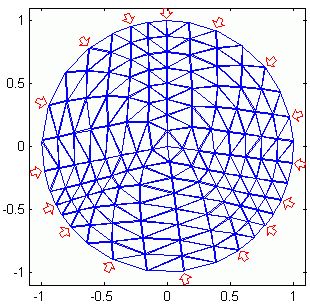
\includegraphics[width= 0.50 \textwidth]{./deform-grille.eps}
\caption{\small 
A finite element mesh deformed in the radial direction to
simulate the effect of model errors for electrode positions.
 }
 \label{fig:deform}
\end{flushright}
\end{figure}

Simulations of model error were conducted and evaluated as
to whether they implemented the happy transform, as shown
in Fig. \ref{fig:deform}.
Of 400 images, approximate 1\% showed this effect. 

%
% FIGURE: Model mismatch images
%
\begin{figure}[th]
\begin{flushright}
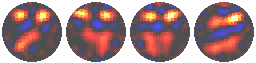
\includegraphics[width= 0.50 \textwidth]{./deform.eps}
\caption{\small 
Sample images reconstucted from a deformed finite element
mesh. Some images were chosen which implement the happy
transform, while others were chosen because they appeared
humourous.
 }
 \label{fig:deform}
\end{flushright}
\end{figure}


\section{
 Discussion
}

The goal of this document is to illustrate some of the things
that can go wrong with the algorithms provided with EIDORS.
While the treatment in this document is lighthearted, it
is surprisingly easy to unwittingly develop mathematical
algorithms which are subject to variants of these {\em cheats}.
We hope that these ideas will help clarify the kinds of
possible errors, and help researchers to avoid them.


\References % Harvard style references

\item[]
Adler A and Guardo R
1996
Electrical impedance tomography: regularised imaging and contrast detection 
\textit{IEEE Trans. Med. Imaging} \textbf{15} 170--9

\item[] 
Polydorides N and Lionheart W R B
2002
A Matlab toolkit for three-dimensional electrical impedance
tomography: a contribution to the Electrical Impedance and
Diffuse Optical Reconstruction Software project,
{\it Meas. Sci. Technol.} {\bf 13} 1871--1883 

\item[] 
Polydorides N 
2002
{\it Image reconstruction algorithms for soft-field tomography}
Ph.D. Thesis,
University of Manchester Institute of Science and Technology, U.K. 

\item[] 
Vauhkonen M 
1997
{\it Electrical impedance tomography and prior information}
PhD thesis, University of Kuopio, Finland 

\item[] 
Vauhkonen M
Lionheart W R B
Heikkinen L M
Vauhkonen P J
Kaipio J P 
2000
A MATLAB package for the EIDORS project to reconstruct
two-dimensional EIT images
{\it Physiol. Meas.} 22 107--111 


\endrefs
\end{document}
